\begin{pa} \label{PA:10.1} 
We investigate the limits of several different functions by working with tables and graphs.
\ba
\item Consider the function $f$ defined by 
  $$
  f(x) = 3-x.
  $$
  Complete the following table of values.
  \begin{center}
    \begin{tabular}{|r|c|}
      \hline      
      $x$ & $f(x)$ \\
      \hhline{|=|=|}
      $-0.2$ & \hspace*{1in} \\
      \hline
      $-0.1$ & \hspace*{1in} \\
      \hline
      0.0 & \hspace*{1in} \\
      \hline
      0.1 & \hspace*{1in} \\
      \hline
      0.2 & \hspace*{1in} \\
      \hline
    \end{tabular}
  \end{center}
  What does the table suggest regarding $\lim_{x\to 0}f(x)$?

\item Explain how your results in (a) are reflected in Figure
  \ref{F:10.1.activity.1}. 

  \begin{figure}[ht]
    \begin{center}
      \scalebox{0.8}{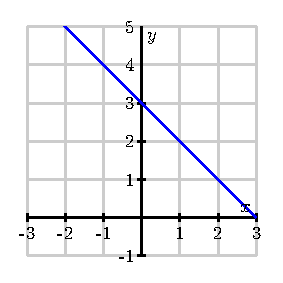
\includegraphics{figures/fig_10_1_activity_3.eps}}
      \caption{The graph of $f(x) = 3-x$.}
      \label{F:10.1.activity.1}
    \end{center}
  \end{figure}
      
      
\item Next, consider $$g(x) = \frac{x}{|x|}.$$
Complete the following table of values near $x = 0$, the point at which $g$ is not defined.
  \begin{center}
    \begin{tabular}{|r|c|}
      \hline      
      $x$ & $g(x)$ \\
      \hhline{|=|=|}
      $-0.1$ & \hspace*{1in} \\
      \hline
      $-0.01$ & \hspace*{1in} \\
      \hline
      $-0.001$ & \hspace*{1in} \\
      \hline
      0.001 & \hspace*{1in} \\
      \hline
       0.01 & \hspace*{1in} \\
      \hline
      0.1 & \hspace*{1in} \\
      \hline
    \end{tabular}
  \end{center}
  What does this suggest about $\lim_{x\to 0}g(x)$?

\item Explain how your results in (c) are reflected in Figure
  \ref{F:10.1.activity.2}. 

  \begin{figure}[ht]
    \begin{center}
      \scalebox{0.8}{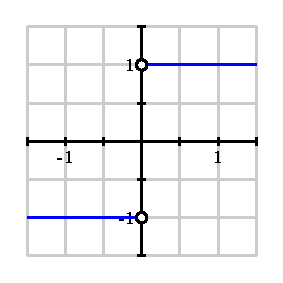
\includegraphics{figures/fig_10_1_activity_2.eps}}
      \caption{The graph of $g(x) = \frac{x}{|x|}$.}
      \label{F:10.1.activity.2}
    \end{center}
  \end{figure}
      
\item Now, let's examine a function of two variables.  Let  
  $$
  f(x,y) = 3 - x - 2y
  $$
  and complete the following table of values.

  \begin{center}
    \begin{tabular}{|r||c|c|c|c|c|}
      \hline
      $x\backslash y$ &$-1$ & $-0.1$ & 0 & 0.1 & 1 \\
      \hhline{|=|=|=|=|=|=|}
      $-1$ & \hspace*{0.5in} & \hspace*{0.5in} & \hspace*{0.5in}  & \hspace*{0.5in} & \hspace*{0.5in} \\
      \hline
      $-0.1$ & & & & & \\
      \hline
      0 & & & & & \\
      \hline
      0.1 & & & & & \\
      \hline
      1 & & & & & \\
      \hline
    \end{tabular}
  \end{center}
  What does the table suggest about $\lim_{(x,y)\to(0,0)} f(x,y)$?

\item Explain how your results in (e) are reflected in Figure
  \ref{F:10.1.activity.4}. Compare this limit to the limit in part (a). How are the limits similar and how are they different?

  \begin{figure}[ht]
    \begin{center}
      \scalebox{0.8}{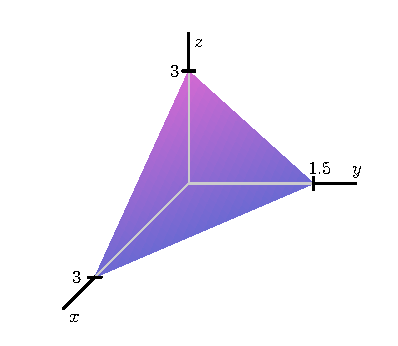
\includegraphics{figures/fig_10_1_limit_contin.eps}}
      \hspace*{0.5in}
      \scalebox{0.8}{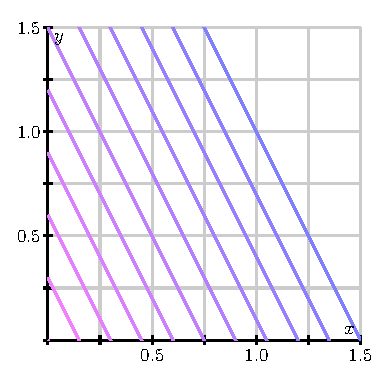
\includegraphics{figures/fig_10_1_cont_contour.eps}}
    \end{center}
      \caption{At left, the graph of $f(x,y) = 3 - x - 2y$; at right, its contour plot.}
      \label{F:10.1.activity.4}
  \end{figure}
      
\item Finally,
  consider
  $$
  g(x,y) = \frac{2xy}{x^2+y^2},
  $$
  which is not defined at $(0,0)$, and complete the following table of values of $g(x,y)$.

  \begin{center}
    \begin{tabular}{|r||c|c|c|c|c|}
      \hline
      $x\backslash y$ &$-1$ &$-0.1$ & 0 & 0.1 & 1 \\
      \hhline{|=|=|=|=|=|=|}
	 $-1$  & \hspace*{0.5in} & \hspace*{0.5in} & \hspace*{0.5in} & \hspace*{0.5in} & \hspace*{0.5in} \\
      \hline
      $-0.1$ & & & & & \\
      \hline
      0  &  &  & --- & & \\
      \hline
       0.1 & & & & & \\
      \hline
      1  & &  & & &  \\
      \hline
    \end{tabular}
  \end{center}
  What does this suggest about $\lim_{(x,y)\to(0,0)} g(x,y)$?

\item Explain how your results are reflected in Figure
  \ref{F:10.1.activity.5}. Compare this limit to the limit in part (b). How are the results similar and how are they different?

  \begin{figure}[ht]
    \begin{center}
      \scalebox{0.8}{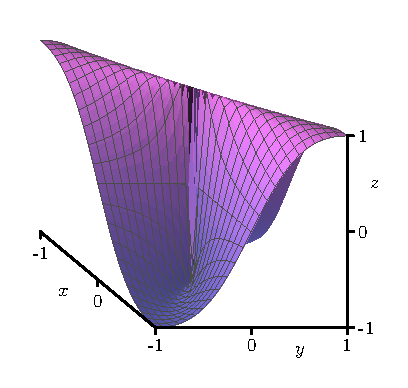
\includegraphics{figures/fig_10_1_limit_disc.eps}}
      \hspace*{0.5in}
      \scalebox{0.8}{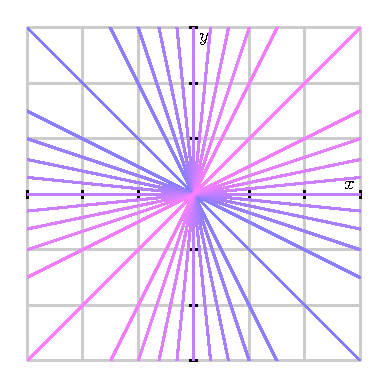
\includegraphics{figures/fig_10_1_limit_contour.eps}}
    \end{center}
      \caption{At left, the graph of $g(x,y) = \frac{2xy}{x^2+y^2}$; at right, its contour plot.}
      \label{F:10.1.activity.5}
  \end{figure}
      
    \ea


\end{pa} 

\begin{activitySolution}
\ba
\item The completed table is below. 
  \begin{center}
    \begin{tabular}{|r|c|}
      \hline      
      $x$ & $f(x)$ \\
      \hhline{|=|=|}
      $-0.2$ & 3.2 \\
      \hline
      $-0.1$ & 3.1 \\
      \hline
      0.0 & 3.0 \\
      \hline
      0.1 & 2.9 \\
      \hline
      0.2 & 2.8 \\
      \hline
    \end{tabular}
  \end{center}
  The table suggests that the values of $f$ get as close to 3 as we want by letting $x$ get as close to 0 as we need. We conclude that 
$\lim_{x\to 0}f(x) = 3$.

\item The graph shows that the points $(x,f(x))$ get as close as we want to the point $(0,3)$ as we let $x$ get as close to 0 as we need. 
      
\item The complete table of values is shown below.
  \begin{center}
    \begin{tabular}{|r|c|}
      \hline      
      $x$ & $g(x)$ \\
      \hhline{|=|=|}
      $-0.1$ & $-1$ \\
      \hline 
      $-0.01$ & $-1$ \\
      \hline
      $-0.001$ & $-1$ \\
      \hline
      0.001 & 1 \\
      \hline
       0.01 & 1 \\
      \hline
      0.1 & 1 \\
      \hline
    \end{tabular}
  \end{center}
  This table suggests that no matter how close we take $x$ to 0, the values of $g(x)$ for $x < 0$ and the values of $g(x)$ for $x > 0$ never get closer than 2. This implies that $\lim_{x\to 0}g(x)$ does not exist. 

\item We can see in the figure that the graph of $g$ makes a jump from $-1$ to $1$ as $x$ changes from negative to positive. This jump discontinuity shows that $g$ does not have a limit at $0$. 
      
\item The complete table of values is below.   

  \begin{center}
    \begin{tabular}{|r||c|c|c|c|c|}
      \hline
      $x\backslash y$ &$-1$ & $-0.1$ & 0 & 0.1 & 1 \\
      \hhline{|=|=|=|=|=|=|}
      $-1$ 	&5 	&4.2 	&4		&3.8 &2 \\
      \hline
      $-0.1$ &5.1 	&3.3 	&3.1 	&2.9 &1.1 \\
      \hline
      0 		&5 	&3.2 	&3 	&2.8 &1 \\
      \hline
      0.1 		&4.9 	&3.1	&2.9 	&2.7 &0.9 \\
      \hline
      1 		&4 	&2.2 	&2 	&1.8 &0 \\
      \hline
    \end{tabular}
  \end{center}
  The values of $f(x,y)$ appear to be approaching 3 as $x$ and $y$ both approach $0$. This suggests that $\lim_{(x,y)\to(0,0)} f(x,y) = 3$.

\item The graph of the surface for $f$ seems to show that the values of $f(x,y)$ approach $3$ as closely as we like as $x$ and $y$ both approach 0. Both $f(x,y) = 3-x-2y$ and $f(x) = 3-x$ are linear functions, so both are continuous everywhere. However, there are only 2 ways as single variable $x$ can approach 0 (from above and from below), while there are many ways that a point $(x,y)$ can approach $(0,0)$. 
      
\item The complete table of values for $g(x,y)$ to three decimal places is below.

  \begin{center}
    \begin{tabular}{|r||c|c|c|c|c|}
      \hline
      $x\backslash y$ &$-1$ &$-0.1$ & 0 & 0.1 & 1 \\
      \hhline{|=|=|=|=|=|=|}
	 $-1$  & 1 & 0.198 & 0 & $-0.198$ & $-1$ \\
      \hline
      $-0.1$ &0.198 &1 &0 &$-1$ &$-0.198$ \\
      \hline
      0  &0  &0  & --- &0 &0 \\
      \hline
       $0.1$ &$-0.198$ &$-1$ &0 &$1$ &$0.198$ \\
      \hline
      $-1$  & $-1$ & $-0.198$ & 0 & $0.198$ & $1$ \\
      \hline
    \end{tabular}
  \end{center}
  The values of $g(x,y)$ are all 0 if $x=0$ or $y=0$. This seems to imply that $g$ has a limit of $0$ at $(0,0)$. However, if $x=y$ we have $g(x,x) = 1$. So the values of $g(x,y)$ do not all get close to the same number as $(x,y)$ approaches $(0,0)$. We conclude that $\lim_{(x,y)\to(0,0)} g(x,y)$ does not exist. 

\item The graph of the surface for $g(x,y) = \frac{2xy}{x^2+y^2}$ seems to show the jump from the values of 0 when $x=0$ or $y=0$ and 1 when $x=y$. This is similar to the graph of $g(x) = \frac{x}{|x|}$ in that there is a jump discontinuity. While $g(x) = \frac{x}{|x|}$ has different one-sided limits at $(0,0)$, it looks like $g(x,y) = \frac{2xy}{x^2+y^2}$ has different limits as $(x,y)$ approaches $(0,0)$ along different paths. 


      
    \ea


\end{activitySolution}

\afterpa 